\documentclass[conf]{new-aiaa}
% for journal papers
%\documentclass[journal]{new-aiaa}
\usepackage[utf8]{inputenc}

\usepackage[version=4]{mhchem}
\usepackage{siunitx}
\usepackage{longtable,tabularx}
\setlength\LTleft{0pt} 
\usepackage{amsmath,amssymb}
\usepackage{graphicx} 
\usepackage{algorithm}
\usepackage{subfig} 
\usepackage{bm}

\title{Paul's paper workflow}

\author{First A. Author\footnote{Insert Job Title, Department Name, Address/Mail Stop, and AIAA Member Grade (if any) for first author.} and Second B. Author Jr.\footnote{Insert Job Title, Department Name, Address/Mail Stop, and AIAA Member Grade (if any) for second author.}}
\affil{Business or Academic Affiliation 1, City, State, Zip Code}
\author{Third C. Author\footnote{Insert Job Title, Department Name, Address/Mail Stop, and AIAA Member Grade (if any) for third author.}}
\affil{Business or Academic Affiliation 2, City, Province, Zip Code, Country}
\author{Fourth D. Author\footnote{Insert Job Title, Department Name, Address/Mail Stop, and AIAA Member Grade (if any) for fourth author (etc.).}}
\affil{Business or Academic Affiliation 2, City, State, Zip Code}

\begin{document}
	
\maketitle

		\begin{abstract}
			This document describes how to set up the workflow for a paper collaborating with Paul.
		\end{abstract}				
	
	\input{sec-nomenclature}
	\section{Introduction}
\label{sec:intro}

\lettrine{T}his document describes the things you need to set up to follow Paul's workflow for writing papers. Here's the software you need to get started:
\begin{enumerate}
\item LaTeX distribution that enables you to run \texttt{latex}, \texttt{pdflatex}, \texttt{bibtex}, \texttt{dvips}, and \texttt{ps2pdf} from the command line,
\item text editor (I use Emacs),
\item Bibtex reference manager (I use JabRef (\url{jabref.org}) because it's based on Java so it's cross platform),
\item Dropbox for sharing a folder.
\end{enumerate}
There are certainly plenty of ways to share LaTeX documents and papers. This is just what's worked for me. I have a directory structure for a paper with the following directories:
\begin{itemize}
\item \texttt{paper\_v0}, where the paper tex files are along with a \texttt{figs} directory; if big changes happen, I might make a new \texttt{paper\_vX} folder
\item \texttt{references}, where I keep PDFs of papers I'm referencing
\item \texttt{code}, where I keep scripts for numerical experiments (helps reproducibility and recreating figures)
\item \texttt{arxiv}, I make a separate folder for the version I put on arXiv
\item \texttt{reviewer\_response}, where I keep a text file of the initial reviews and a LaTeX file with reviewer responses
\item \texttt{latexdiff}, when I submit a revision I include the results of \texttt{latexdiff} (see example syntax in folder)
\item \texttt{paper\_r0}, a folder for the revision; this usually begins as a duplicate of \texttt{paper\_v0}
\end{itemize}
	\section{LaTeX}
\label{sec:latex}

\noindent There are several text editors that include tools for working with LaTeX. I don't really like any of them. Emacs has a natural ``latex-mode'' that does some syntax highlighting---and there's a lot you can do the integrate LaTeX with Emacs (see, for example, Nick Higham's blog: \url{https://nickhigham.wordpress.com/category/latex/}). However, I don't use any of it. I just use Emacs to create~.tex documents. 

I compile a completed~.tex file with a Makefile that executes LaTeX commands. From the command line, just type \texttt{make}. My Makefile's contain two ways to compile: (i) with \texttt{latex} and (ii) with \texttt{pdflatex}. The latter is preferred, but some journal templates need to use the former (for some reason). 

Here are some sample environments I use regularly in papers. See Algorithm \ref{alg:0} and Figure \ref{fig:0} with Subfigures \ref{fig:sub0} and \ref{fig:sub1}. 

\begin{algorithm}
Given some stuff, do the following:
\begin{enumerate}
\itemsep0em
\item Step 1
\item Step 2
\end{enumerate}
\caption{My favorite algorithm}
\label{alg:0}
\end{algorithm}

\begin{figure}[!h]
\centering
\subfloat[Label 1]{
\label{fig:sub0}
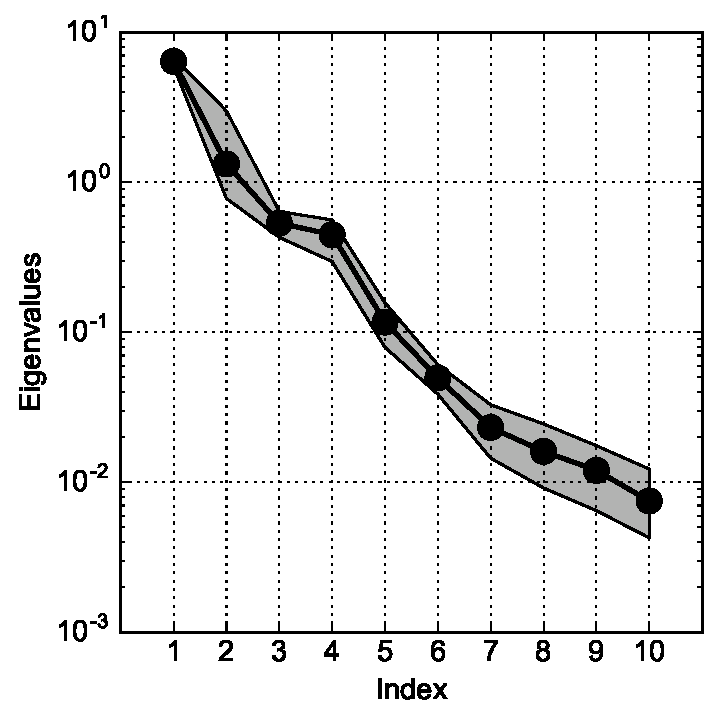
\includegraphics[width=0.42\textwidth]{figs/evals_drag.eps}%
}
\hfil
\subfloat[Label 2]{
\label{fig:sub1}
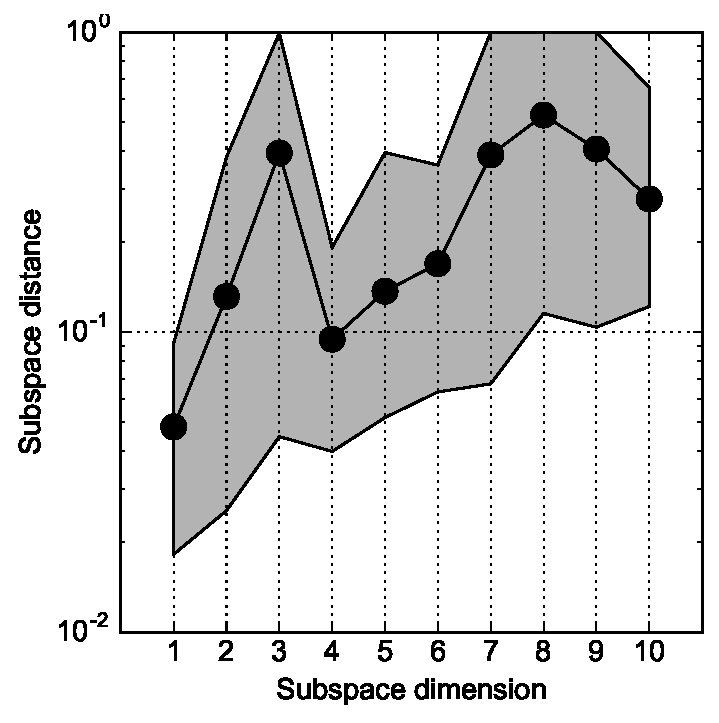
\includegraphics[width=0.42\textwidth]{figs/subspace_drag.eps}%
}
\caption{And this is where you put the caption}
\label{fig:0}
\end{figure}

I usually make figures in the code directory and manually move them to the \texttt{paper\_v0/figs} directory. That way, if I change the figure in the code because I'm playing around, then it doesn't immediately change the paper figure.

	\section{Code and examples}
\label{sec:examples}

\noindent I put all the scripts that run the numerical experiments and the data they generate (assuming it's a resonable size) in the \texttt{code} directory. Doing this makes it easier to return to the code that generated a particular figure. I also use \texttt{git} and \url{bitbucket.org} to make the scripts accessible online. See my existing scripts at \url{bitbucket.org/paulcon}. 

	\section{Bibtex and references}

\noindent I use Jabref as a reference manager for citations like this one~\cite{asmbook}. To get the bibtex records for papers, I find the paper on its journal's webpage and click something like 'Download citation' that most of the journals have. That's a good place to start, but the bibtex records are often imperfect. 



	\input{sec-AIAA}
	
	\section*{Acknowledgments}
	
	\noindent Thanks to all my coauthors for helping me hone my workflow.
	
	%\section*{References}
	\bibliography{workflow}
	
\end{document}
